\documentclass[border=10pt]{standalone}

\usepackage{tikz}
\usepackage{tikzsymbols}
\usetikzlibrary{calc,patterns,shapes.geometric}

\def\centerarc[#1](#2)(#3:#4:#5){\draw[#1] ($(#2)+({#5*cos(#3)},{#5*sin(#3)})$) arc (#3:#4:#5);}

\begin{document}
	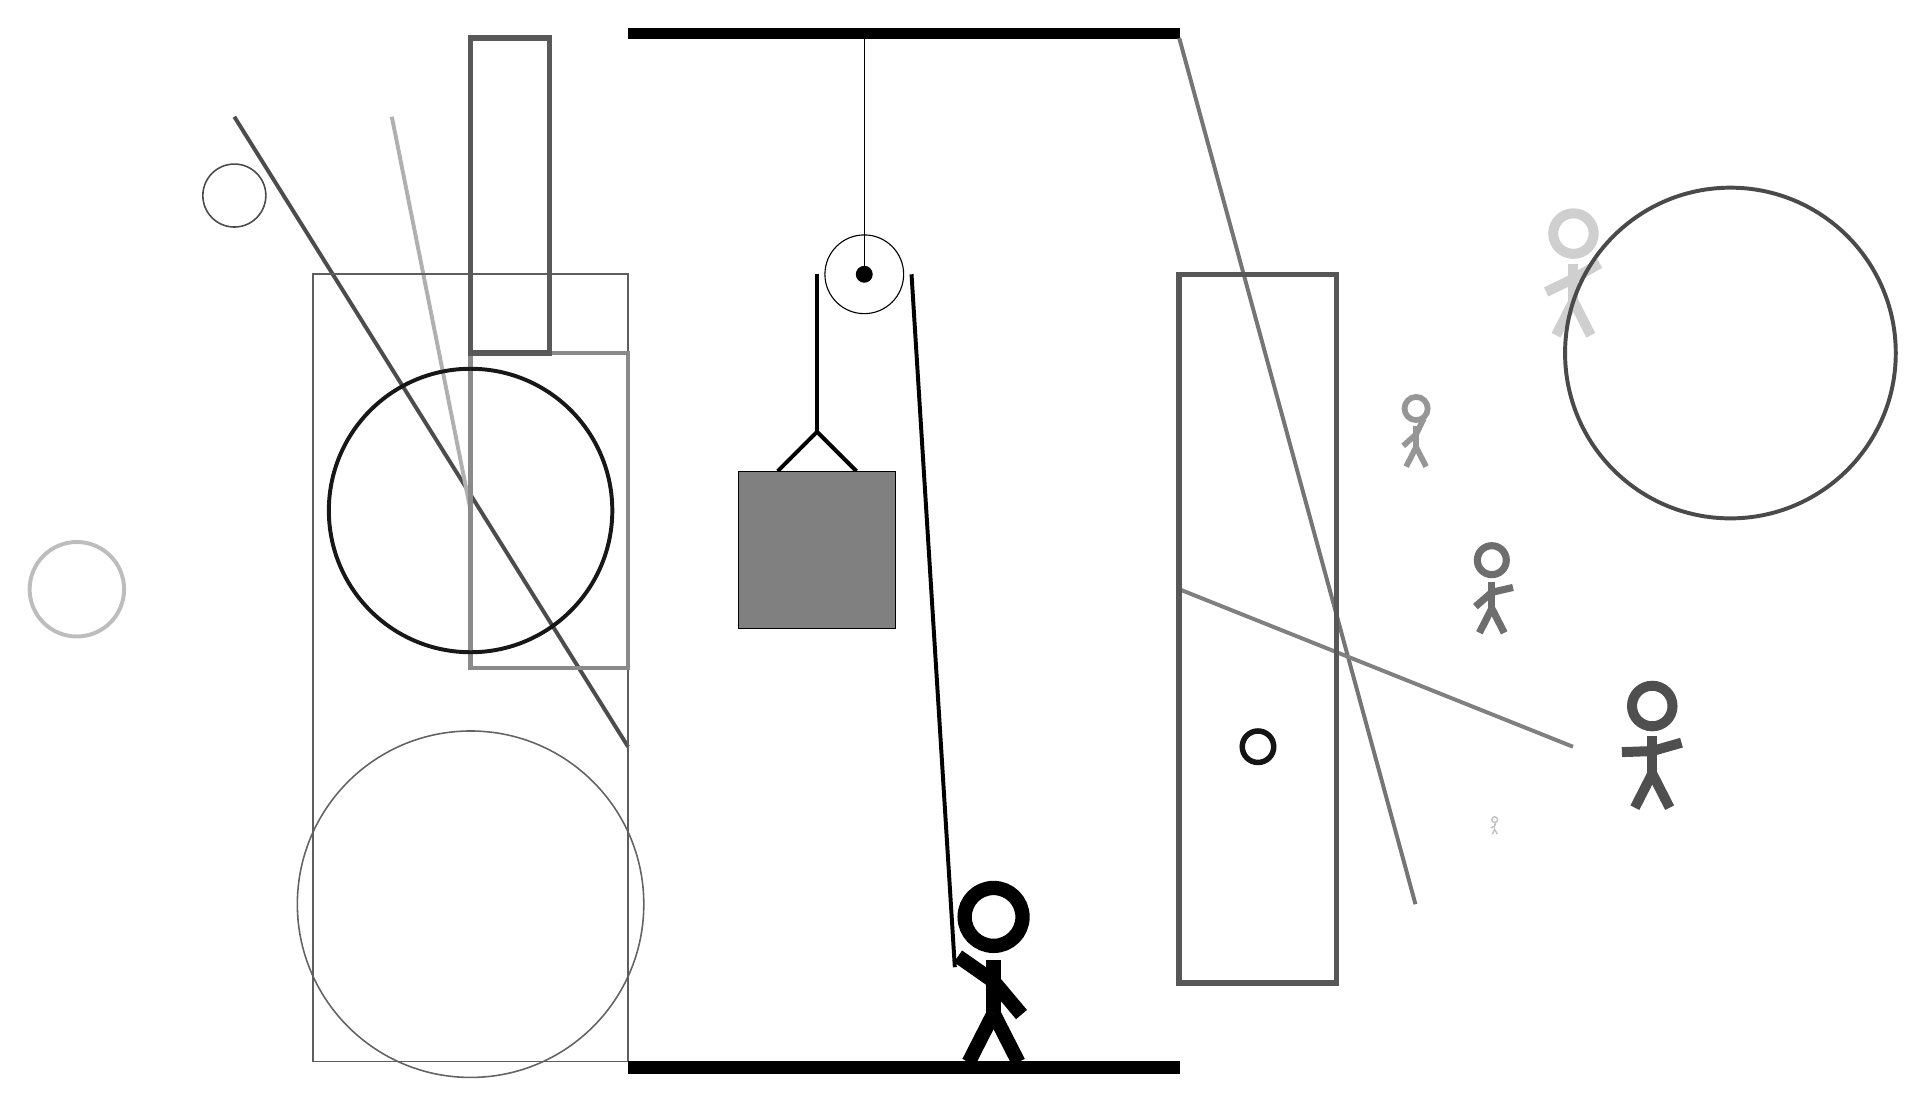
\begin{tikzpicture}
		%%%%% START %%%%%
		
		\draw[fill=black] (-2, 10) rectangle (5, 10.125);
		
		\draw (1, 7) circle (0.5);
		\draw[fill=black] (1, 7) circle (0.1);
		\draw (1, 10) -- (1, 7);
		
		\draw[line width=0.5mm] (-0.1, 4.5) -- (0.4, 5.0) -- (0.9, 4.5);
		\draw[fill=black!50] (-0.6, 4.5) rectangle (1.4, 2.5);
		
		\draw[line width=0.5mm] (0.4, 7) -- (0.4, 5.0);
		\centerarc[line width=0.5mm](1, 7)(0:180:0.6);
		\draw[line width=0.5mm](1.6, 7) -- (2.15, -1.8);
		
		\draw [line width=0.5mm, color=black!26](-9, 3) circle (0.6);
		
		\draw[line width=0.5mm, color=black!54](8, -1) -- (5, 10);
		\node[line width=0.7mm, color=black!24] at (9, 0) {\Strichmaxerl[1][26][76]};
		\node[line width=0.5mm, color=black!41] at (8, 5) {\Strichmaxerl[4][42][64]};
		\draw [line width=0.2mm, color=black!61](-4, -1) circle (2.2);
		\draw [line width=0.2mm, color=black!71](-7, 8) circle (0.4);
		
		\draw[line width=0.5mm, color=black!70](-2, 1) -- (-7, 9);
		
		\draw[line width=0.5mm, color=black!31](-4, 4) -- (-5, 9);
		\draw[line width=0.5mm, color=black!73] (-3, 7) rectangle (-3, 9);
		\draw[line width=0.2mm, color=black!63] (-2, -3) rectangle (-6, 7);
		\draw[line width=0.7mm, color=black!99] (7, 0) rectangle (7, 2);
		
		\draw [line width=0.7mm, color=black!92](6, 1) circle (0.2);
		\node[line width=0.6mm, color=black!57] at (9, 3) {\Strichmaxerl[5][41][13]};
		
		\draw[line width=0.5mm, color=black!50](10, 1) -- (5, 3);
		\draw[line width=0.7mm, color=black!84] (5, -1) rectangle (5, 2);
		\node[line width=0.7mm, color=black!69] at (11, 1) {\Strichmaxerl[7][2][16]};
		
		\draw[line width=0.6mm, color=black!46] (-4, 6) rectangle (-2, 2);
		\draw[line width=0.7mm, color=black!65] (-4, 10) rectangle (-3, 6);
		\draw [line width=0.5mm, color=black!91](-4, 4) circle (1.8);
		\draw[line width=0.7mm, color=black!66] (5, 7) rectangle (7, -2);
		\node[line width=0.6mm, color=black!19] at (10, 7) {\Strichmaxerl[7][26][30]};
		\draw [line width=0.5mm, color=black!71](12, 6) circle (2.1);
		
		\node at (2.6, -1.9) {\Strichmaxerl[10][-35][-50]};
		
		\draw[fill=black] (-2, -3) rectangle (5, -3.15);
		
		%%%%% END %%%%%
	\end{tikzpicture}
\end{document}